%if printing on both sides of a page add 'twopage' to the [...] below
\documentclass[11pt,openright]{report} 
\usepackage{graphicx}
\usepackage{color}
\usepackage{tocbibind}
%\usepackage{algorithm2e} % must be included before unlv-thesis
\usepackage[linesnumbered,ruled]{algorithm2e}
\SetKwProg{Fn}{Function}{}{}
\usepackage{subcaption}
\usepackage{fancyhdr}
\usepackage{unlv-thesis}

\graphicspath{{./images/}, {./results/}}
\usepackage{hyperref}
\hypersetup{
	colorlinks=false, %set true if you want colored links
	linktoc=all,     %set to all if you want both sections and subsections linked
	linkcolor=blue,  %choose some color if you want links to stand out
}
%%%
%%% Choose either \phdthesis or \mastersthesis
\mastersthesis
%\phdthesis

%%%
%%% opens all chapters on right hand sides (needed for double sided printing)
\rightchapter
%%% add \twosided if you are printing on both sides
%\twosided
%%%
%%% Choose the spacing for the thesis: \singlespace, \oneandhalfspace or \doublespace
%\oneandhalfspace
%\singlespace
\doublespace

\makeindex

%%%
%%% The name of your thesis and your own name. Title must be in all
%%% caps and in an inverted triangle
\thesistitle{SECURE DECENTRALIZED STORAGE USING BLOCKCHAIN}
\thesistitlelowercase{Secure Decentralized Storage Using Blockchain}
\thesisauthor{Vinay Kumar Calastry Ramesh}

%%%
%%% Add your previous degrees here
\thesisauthorpreviousdegrees{
Bachelor of Technology in Computer Science\\ \vspace*{-0.12in}
Jawaharlal Nehru Technological University, Hyderabad\\ \vspace*{-0.12in}
2014}

%%%
%%% Month and Year to appear on the thesis
\thesismonth{May} 
\thesisyear{2019}
\copyrightyear{2019}

%%%
%%% The size of the committee: chair + other members + college rep (normally 4)
%%% use \chair{}, \memberone{}, \membertwo{}, \memberthree{}, \colleferep{}
\thesiscommitteesize{4}
%\signatures{}   % will generate 'signatures on the approval page' grad college does 
%not like this, so don't do that in their version
\chair{Yoohwan\ Kim, Ph.D.}
\memberone{Laxmi\ Gewali, Ph.D.}
\membertwo{Fatma\ Nasoz, Ph.D.}
\collegerep{Ge\ Lin\ Kan, Ph.D.}

%----------------------- Macros ----------------------------------------- 

%\newcounter{defcounter}
%\setcounter{defcounter}{1}
%\newcounter{excounter}
%\setcounter{excounter}{1}
%\newcounter{propcounter}
%\setcounter{propcounter}{1}
%\newcounter{lemmacounter}
%\setcounter{lemmacounter}{1}
%\newcounter{theoremcounter}
%\setcounter{theoremcounter}{1}                    
\newcommand{\mytheoremcounter}{section}
\newcommand{\cheapHack}{ }
\newcommand{\BAPrn}{BAP$_{\mbox{r}}$}
\newcommand{\BAPr}{BAP$_{\mbox{r}}$\ }
\newcommand{\BAPsn}{BAP$_{\mbox{s}}$}
\newcommand{\BAPs}{BAP$_{\mbox{s}}$\ }
\newcommand{\BAPsrn}{BAP$_{\mbox{sr}}$}
\newcommand{\BAPsr}{BAP$_{\mbox{sr}}$\ }
\newcommand{\BAPucn}{BAP$_{\mbox{sr}}$}
\newcommand{\BAPuc}{BAP$_{\mbox{sr}}$\ }
\newcommand{\BSPrn}{BSP$_{\mbox{r}}$}
\newcommand{\BSPr}{BSP$_{\mbox{r}}$\ }
\newcommand{\BSPsn}{BSP$_{\mbox{s}}$}
\newcommand{\BSPs}{BSP$_{\mbox{s}}$\ }
\newcommand{\BSPsrn}{BSP$_{\mbox{sr}}$}
\newcommand{\BSPsr}{BSP$_{\mbox{sr}}$\ }
\newcommand{\BSPucn}{BSP$_{\mbox{sr}}$}
\newcommand{\BSPuc}{BSP$_{\mbox{sr}}$\ }
\newcommand{\NBAPrn}{NBAP$_{\mbox{r}}$}
\newcommand{\NBAPr}{NBAP$_{\mbox{r}}$\ }
\newcommand{\NBAPsn}{NBAP$_{\mbox{s}}$}
\newcommand{\NBAPs}{NBAP$_{\mbox{s}}$\ }
\newcommand{\NBAPsrn}{NBAP$_{\mbox{sr}}$}
\newcommand{\NBAPsr}{NBAP$_{\mbox{sr}}$\ }
\newcommand{\NBAPucn}{NBAP$_{\mbox{sr}}$}
\newcommand{\NBAPuc}{NBAP$_{\mbox{sr}}$\ }
\newcommand{\fixme}[1]{$\spadesuit$\marginpar{\tiny$\spadesuit$#1}}
\newcommand{\Xhalf}{X_\frac{1}{2}}
\newcommand{\Shalf}{\cS_{\frac{n}{2},n}}
\newcommand{\chih}{\chi_n}
\newcommand{\notchih}{\overline{\chi_n}}
\newcommand{\upsh}{\upsilon_n}
\newcommand{\notupsh}{\overline{\upsilon_n}}
\newcommand{\singlespacing}{\baselineskip 1em}
\newcommand{\onehalfspacing}{\baselineskip 1.25em}
\newcommand{\doublespacing}{\baselineskip 1.75em}
\newcommand{\truedoublespacing}{\baselineskip 2em}
\newcommand{\normalspacing}{\singlespacing}
\newcommand{\Paccept}[1]{{\Pr[#1 = \mathrm{accept}]}}
\newcommand{\Maj}{\mathit{Maj}}
\newcommand{\Nand}{\uparrow}
\newcommand{\Nor}{\downarrow}
\newcommand{\myem}[1]{{\bf #1}}
\newcommand{\reccr}[1]{\overline{\nu}(#1)}
\newcommand{\regcr}[1]{\nu(#1)}
\newcommand{\LOGDCFLclass}{\mathbf{LOGDCFL}}
\newcommand{\NLclass}{\mathbf{NL}}
\newcommand{\ACclass}{\mathbf{AC}}
\newcommand{\NCclass}{\mathbf{NC}}
\newcommand{\SCclass}{\mathbf{SC}}
\newcommand{\RCclass}{\mathbf{RC}}
\newcommand{\coNLclass}{\mathbf{co\!-\!NL}}
\newcommand{\Lclass}{\mathbf{L}}
\newcommand{\Lpoly}{\mathbf{L}_{/\mathrm{poly}}}
\newcommand{\Pclass}{\mathbf{P}}
\newcommand{\BPclass}{\mathbf{P}_{BP}}
\newcommand{\BPwidth}[1]{\mathbf{P}_{BP}^{#1}}
\newcommand{\NPclass}{\mathbf{NP}}
\newcommand{\coNPclass}{\mathbf{coNP}}
\newcommand{\PPclass}{\mathbf{PP}}
\newcommand{\BPPclass}{\mathbf{BPP}}
\newcommand{\ZPPclass}{\mathbf{ZPP}}
\newcommand{\RPclass}{\mathbf{RP}}
\newcommand{\coRPclass}{\mathbf{co\!-\!RP}}
\newcommand{\SigmaP}[1]{\mathbf{\Sigma_{#1}P}}
\newcommand{\PHclass}{\mathbf{PH}}
\newcommand{\PSPACE}{\mathbf{PSPACE}}
\newcommand{\RSPACE}{\mathbf{RSPACE}}
\newcommand{\DSPACE}{\mathbf{DSPACE}}
\newcommand{\imin}{{\mathit{min}}}
\newcommand{\imax}{{\mathit{max}}}
\newcommand{\gbf}{{\mathbf{g}}}
\newcommand{\zbf}{{\mathbf{z}}}
\newcommand{\wbf}{{\mathbf{w}}}
\newcommand{\vbf}{{\mathbf{v}}}
\newcommand{\xbf}{{\mathbf{v}}}
\newcommand{\onebf}{{\mathbf{1}}}
\newcommand{\zerobf}{{\mathbf{0}}}
\newcommand{\uvec}{\vec{u}}
\newcommand{\vvec}{\vec{v}}
\newcommand{\xvec}{\vec{x}}
\newcommand{\Deltap}{\Delta^\prime}
\newcommand{\Sigmap}{{\Sigma^\prime}}
\newcommand{\alphap}{\alpha^\prime}
\newcommand{\betap}{\beta^\prime}
\newcommand{\betapp}{\beta^{\prime\prime}}
\newcommand{\gammap}{\gamma^\prime}
\newcommand{\mup}{\mu^\prime}
\newcommand{\mupp}{\mu^{\prime\prime}}
\newcommand{\nubar}{{\overline{\nu}}}
\newcommand{\nubars}{\nubar^*}
\newcommand{\nus}{\nu^*}
\newcommand{\betas}{\beta^*}
\newcommand{\deltas}{\delta^*}
\newcommand{\deltap}{\delta^\prime}
\newcommand{\deltapp}{\delta^{\prime\prime}}
\newcommand{\lambdabar}{\overline{\lambda}}
\newcommand{\lambdap}{\lambda^\prime}
\newcommand{\lambdapp}{\lambda^{\prime\prime}}
\newcommand{\pip}{\pi^\prime}
\newcommand{\pipp}{{\pi^{\prime\prime}}}
\newcommand{\Psip}{\Psi^\prime}
\newcommand{\psip}{\psi^\prime}
\newcommand{\phip}{\phi^\prime}
\newcommand{\sigmap}{\sigma^\prime}
\newcommand{\etap}{\eta^\prime}
\newcommand{\etapp}{{\eta^{\prime\prime}}}
\newcommand{\epsilonp}{{\epsilon^\prime}}
\newcommand{\epsilonpp}{\epsilon^{\prime\prime}}
\newcommand{\epsilonppp}{\epsilon^{\prime\prime\prime}}
\newcommand{\ap}{a^\prime}
\newcommand{\bp}{b^\prime}
\newcommand{\cp}{c^\prime}
\newcommand{\up}{u^\prime}
\newcommand{\fp}{f^\prime}
\newcommand{\ep}{e^\prime}
\newcommand{\gp}{g^\prime}
\newcommand{\ip}{i^\prime}
\newcommand{\jp}{j^\prime}
\newcommand{\mpr}{m^\prime}
\newcommand{\np}{n^\prime}
\newcommand{\op}{o^\prime}
\newcommand{\qp}{q^\prime}
\newcommand{\rp}{r^\prime}
\newcommand{\spr}{s^\prime}
\newcommand{\tp}{t^\prime}
\newcommand{\gpp}{g^{\prime\prime}}
\newcommand{\ipp}{i^{\prime\prime}}
\newcommand{\jpp}{j^{\prime\prime}}
\newcommand{\epp}{e^{\prime\prime}}
\newcommand{\qpp}{q^{\prime\prime}}
\newcommand{\rpp}{r^{\prime\prime}}
\newcommand{\vp}{v^\prime}
\newcommand{\ypp}{y^{\prime\prime}}
\newcommand{\xpp}{x^{\prime\prime}}
\newcommand{\zp}{z^\prime}
\newcommand{\hp}{{h^\prime}}
\newcommand{\lp}{{l^\prime}}
\newcommand{\zpp}{{z^{\prime\prime}}}
\newcommand{\kp}{{k^\prime}}
\newcommand{\Dp}{{D^\prime}}
\newcommand{\Pp}{P^\prime}
\newcommand{\Ppp}{P^{\prime\prime}}
\newcommand{\Qp}{Q^\prime}
\newcommand{\Qpp}{Q^{\prime\prime}}
\newcommand{\Spr}{S^\prime}
\newcommand{\Tp}{T^\prime}
\newcommand{\Ep}{E^\prime}
\newcommand{\Dbar}{\overline{D}}
\newcommand{\Lp}{L^\prime}
\newcommand{\Lpp}{L^{\prime\prime}}
\newcommand{\Lbar}{\overline{L}}
\newcommand{\Lhat}{\widehat{L}}
\newcommand{\Ltilde}{\tilde{L}}
\newcommand{\Lcap}{{L^\cap}}
\newcommand{\Lcup}{{L^\cup}}
\newcommand{\Lpbar}{\overline{\Lp}}
\newcommand{\Mp}{M^\prime}
\newcommand{\Mpp}{M^{\prime\prime}}
\newcommand{\Mbar}{\overline{M}}
\newcommand{\Np}{N^\prime}
\newcommand{\Npp}{N^{\prime\prime}}
\newcommand{\Rp}{R^\prime}
\newcommand{\xbar}{\bar{x}}
\newcommand{\xp}{x^\prime}
\newcommand{\yp}{y^\prime}
\newcommand{\Uhat}{\widehat{U}}
\newcommand{\Up}{U^\prime}
\newcommand{\Upp}{U^{\prime\prime}}
\newcommand{\Vp}{V^\prime}
\newcommand{\Vhat}{\widehat{V}}
\newcommand{\Vbar}{\overline{V}}
\newcommand{\Ap}{{A^\prime}}
\newcommand{\App}{{A^{\prime\prime}}}
\newcommand{\Cp}{C^\prime}
\newcommand{\Fp}{F^\prime}
\newcommand{\Gp}{G^\prime}
\newcommand{\Gtilde}{\tilde{G}}
\newcommand{\Fpp}{F^{\prime\prime}}
\newcommand{\Zf}{{\mathbb{Z}}}
\newcommand{\Qf}{{\mathbb{Q}}}
\newcommand{\Rf}{{\mathbb{R}}}
\newcommand{\Cf}{{\mathbb{C}}}
\providecommand{\mathbb}[1]{\Bbb{#1}}
\newcommand{\qacc}{q^{acc}}
\newcommand{\qrej}{q^{rej}}
\newcommand{\qnon}{q^{non}}
\newcommand{\Qadd}{Q_{add}}
\newcommand{\Qacc}{Q_{acc}}
\newcommand{\Qrej}{Q_{rej}}
\newcommand{\Qnon}{Q_{non}}
\newcommand{\Qhalt}{Q_{halt}}
\newcommand{\Qjunk}{Q_{junk}}
\newcommand{\Qaccp}{{Q_{acc}^\prime}}
\newcommand{\Qrejp}{{Q_{rej}^\prime}}
\newcommand{\Qnonp}{{Q_{non}^\prime}}
\newcommand{\Qhaltp}{{Q_{halt}^\prime}}
\newcommand{\Qjunkp}{{Q_{junk}^\prime}}
\newcommand{\Qaccpp}{{Q_{acc}^{\prime\prime}}}
\newcommand{\Qrejpp}{{Q_{rej}^{\prime\prime}}}
\newcommand{\Qnonpp}{{Q_{non}^{\prime\prime}}}
\newcommand{\Qjunkpp}{{Q_{junk}^{\prime\prime}}}
\newcommand{\Cacc}{C_{acc}}
\newcommand{\Crej}{C_{rej}}
\newcommand{\Cnon}{C_{non}}
\newcommand{\Eacc}{E_{acc}}
\newcommand{\Erej}{E_{rej}}
\newcommand{\Enon}{E_{non}}
\def\cent{{\hbox{\rm\rlap/c}}}
\newcommand{\centp}{{\cent}^\prime}
\newcommand{\Bra}[1]{{\langle{#1}|}}
\newcommand{\Ket}[1]{{|{#1}\rangle}}
\newcommand{\BraKet}[2]{{\langle{#1}|{#2}\rangle}}
\newcommand{\iprod}[2]{{\langle{#1},{#2}\rangle}}
\newtheorem{theorem}{{\bf Theorem}}[\mytheoremcounter]
\newtheorem{lemma}[theorem]{{\bf Lemma}}
\newtheorem{aside}[theorem]{{\bf Aside}}
%\newtheorem{claim}[theorem]{{\bf Claim}}
\newtheorem{example}[theorem]{{\bf Example}}
\newtheorem{question}[theorem]{{\bf Question}}
\newtheorem{answer}[theorem]{{\bf Answer}}
\newtheorem{conjecture}[theorem]{{\bf Conjecture}}
\newtheorem{proposition}[theorem]{{\bf Proposition}}
\newtheorem{property}[theorem]{{\bf Property}}
\newtheorem{corollary}[theorem]{{\bf Corollary}}
\newtheorem{observation}[theorem]{{\bf Observation}}
%\newtheorem{fact}[theorem]{{\bf Fact}}
\newtheorem{definition}[theorem]{{\bf Definition}}
\newtheorem{remark}[theorem]{{\bf Remark}}
\newtheorem{thoughts}[theorem]{{\bf Thoughts}}
\newenvironment{proof}{ \begin{trivlist} 
                        \item \vspace{-\topsep} \noindent{\bf Proof:}\ }
                      {\rule{5pt}{5pt}\end{trivlist}}
\newcommand{\Subcase}[2]{\noindent{\bf Subcase #1:}#2}
\newcommand{\Half}{\frac{1}{2}}
\newcommand{\RtHalf}{\frac{1}{\sqrt{2}}}
\newcommand{\cA}{{\mathcal{A}}}
\newcommand{\cC}{{\mathcal{C}}}
\newcommand{\cE}{{\mathcal{E}}}
\newcommand{\cF}{{\mathcal{F}}}
\newcommand{\cH}{{\mathcal{H}}}
\newcommand{\cI}{{\mathcal{I}}}
\newcommand{\cK}{{\mathcal{K}}}
\newcommand{\cL}{{\mathcal{L}}}
\newcommand{\cM}{{\mathcal{M}}}
\newcommand{\cO}{{\mathcal{O}}}
\newcommand{\cP}{{\mathcal{P}}}
\newcommand{\cR}{{\mathcal{R}}}
\newcommand{\cS}{{\mathcal{S}}}
\newcommand{\cU}{{\mathcal{U}}}
\newcommand{\Span}{{\mathit{Span}}}
\newcommand{\Ch}[2]{{#1 \choose #2}}
\newcommand{\Ul}[1]{{\underline{#1}}}
\newcommand{\Floor}[1]{{\lfloor #1 \rfloor}}
\newcommand{\ignore}[1]{}
\newcommand{\noignore}[1]{#1}

\newcommand{\RMO}{\mathbf{RMO}}
\newcommand{\UMO}{\mathbf{UMO}}
\newcommand{\RMOe}{\mathbf{RMO}_\epsilon}
\newcommand{\RMM}{\mathbf{RMM}}
\newcommand{\UMM}{\mathbf{UMM}}
\newcommand{\RMMe}{\mathbf{RMM}_\epsilon}

\newcommand{\MOQFA}{\mathbf{MOQFA}}
\newcommand{\MOQFAe}{\mathbf{MOQFA}_\epsilon}
\newcommand{\MMQFA}{\mathbf{MMQFA}}
\newcommand{\MMQFAe}{\mathbf{MMQFA}_\epsilon}
\newcommand{\GQFA}{\mathbf{GQFA}}
\newcommand{\GQFAe}{\mathbf{GQFA}_\epsilon}

\newcommand{\REG}{\mathbf{REG}}
\newcommand{\PFA}{\mathbf{PFA}}
\newcommand{\PFAe}{\mathbf{PFA}_\epsilon}
\newcommand{\GFA}{\mathbf{GFA}}

% Code environment
\newcommand{\Foreach}[2]{\\{\bf\tt{for\ each}} $#1$ {\bf\tt{do}}\+ #2
\- \\ {\bf\tt{rof}}}
\newcommand{\Forloop}[2]{\\{\bf\tt{for}} $#1$ {\bf\tt{do}}\+ #2
\- \\ {\bf\tt{rof}}}
\newcommand{\Ifthen}[2]{\\{\bf\tt{if}} $#1$ {\bf\tt{then}}\+ #2
\- \\ {\bf\tt{fi}}}
\newcommand{\Ifelse}[3]{\\{\bf\tt{if}} $#1$ {\bf\tt{then}}\+ #2
\- \\ {\bf\tt{else}}\+ #3 \- \\ {\bf\tt{fi}}}
\newcommand{\Stmt}[1]{\\$#1$;}
\newcommand{\StartStmt}[1]{\+\kill$#1$;}
\newenvironment{pseudocode}{\begin{tabbing} 
\ \ \ \ \=\ \ \ \ \=\ \ \ \ \=\ \ \ \ \=\ \ \ \ \=\ \ \ \ \=\ \ \ \ \=\
\ \ \ \= } {\end{tabbing}}

% Moving proofs around
% #1 = proof \name   #2 = appendix ref    #3 = proof
\providecommand{\SaveProof}[3]{#3}
% #1 = proof \name   #2 = appendix ref    #3 = proof    #4 = sketch
\providecommand{\SketchProof}[4]{#3}
% #1 = proof \name   #2 = appendix label  #3 = title
\providecommand{\AppendixProof}[3]{}

\newcommand{\MoveProofsToAppendix}{\include{movemacs}}

% Short equation separator
\newcommand{\ShortSep}{\\ & &}
\newcommand{\LongSep}{}
\providecommand{\DefSep}{\LongSep}
\newcommand{\UseShortSep}{\renewcommand{\DefSep}{\ShortSep}}


% select abstract mechanism
\newcommand{\UseAbstract}[2]{#1}
\newcommand{\UseOtherAbstract}{\include{absselect}}

% EVIL stuff to make it fit for 10 page limit (two lines per page extra)
\newcommand{\StretchPage}{ \addtolength{\textheight}{0.05\textheight}
                           \addtolength{\topmargin}{-0.03\textheight}
                         }

% figure macro

\newcommand{\DoFigure}[4]{
                          \begin{figure}[ht]
\setlength{\topsep}{-10pt}
\setlength{\parsep}{0pt}
\setlength{\partopsep}{0pt}
\setlength{\parskip}{0pt}
                            \begin{center}
                              \ \includegraphics[scale=#2]{#1}\ 
                            \end{center}
                            \caption{#3\label{#4}}
                          \end{figure}
                         }

\newcommand{\DoBiFigure}[5]{
                          \begin{figure}[ht]
\setlength{\topsep}{-10pt}
\setlength{\parsep}{0pt}
\setlength{\partopsep}{0pt}
\setlength{\parskip}{0pt}
                            \begin{center}
                              \mbox{\ \includegraphics[scale=#3]{#1}\ 
                                    \hspace{1.0in}
                                    \ \includegraphics[scale=#3]{#2}\ }
                            \end{center}
                            \caption{#4\label{#5}}
                          \end{figure}
                         }

\newcommand{\DoDiFigure}[8]{ 
                          \begin{figure}[ht]
\setlength{\topsep}{-10pt}
\setlength{\parsep}{0pt}
\setlength{\partopsep}{0pt}
\setlength{\parskip}{0pt}
                            \begin{center}
                              \begin{minipage}[b]{0.35\linewidth}
                                \begin{center}
                                  \includegraphics[scale=#2]{#1}
                                \end{center}
                                \caption{#3\label{#4}}
                              \end{minipage}
                              \hspace{1.0in}
                              \begin{minipage}[b]{0.35\linewidth}
                                \begin{center}
                                  \includegraphics[scale=#6]{#5}
                                \end{center}
                                \caption{#7\label{#8}}
                              \end{minipage}
                            \end{center}
                          \end{figure}
                         }

\newcommand{\DoTable}[3]{
                          \begin{table}[ht]
                            \begin{center}
                              #1
                            \end{center}
                            \caption{#2\label{#3}}
                          \end{table}
                         }


\newcommand{\pseudosection}[1]{\vspace{\baselineskip}
\noindent{\sffamily\bfseries #1}\vspace{0.5\baselineskip}}
\newcommand{\mycaption}[3]{
 \begin{center}
   \parbox{0.90\columnwidth}{\caption[#1]{
     \setlength{\baselineskip}{1.3\baselineskip}
     #2}\label{#3}}
 \end{center}}



%---------------------- Thesis starts here ------------------------------

% The organization should be as follows, as per our online guidelines:
% page (not numbered): title page
% page (not numbered): copyright statement (this page is optional)
% page ii: approval page, but do not inlcude it until the grad college says ok.
% page iii:  abstract
% acknowledgments
% preface
% table of contents
% list of tables 
% list of figures
% page 1 -> ???: main body of text
% exhibits (what ever that is)
% appendices
% bibliography,
% author's CV. 

% everything after main body should have regular page numbers, 
% everything before should have roman numeral in small letters.
\begin{document}
\thesistitlepage
\copyrightpage

\newpage
%% here goes the approval page - uncomment the following line when you 
%% get an ok from the graduate college:
%%
%% \approvalpage for the page that people need to sign
%%
%% \electronicapprovalpage for the page that needs to be used when submitting the PDF

%\approvalpage
\electronicapprovalpage


\begin{thesisabstract}
High utility item set mining is an important data mining problem which considers profit factors besides quantity from the transactional database. It helps find the most valuable products/items that are difficult to track using only the mere frequent data mining set. An item that has a high-profit value might be rare in the transactional database despite its tremendous importance. While there are many existing algorithms which generate comparatively large candidate sets while finding high utility itemsets, the major focus is to reduce the computational time significantly with the introduction of pruning strategies. Another aspect of high utility itemset mining is to compute the large dataset. There are very few algorithms that can handle large dataset to find high utility itemset mining in a parallel (distributed) system.

In this thesis, there are two proposed methods: High utility itemset mining using pruning strategies approach (HUI-PR) and Parallel EFIM (EFIM-Par). In the method I, the proposed algorithm constructs the candidate sets in the form of a tree structure, which traverses the itemsets with high transaction weighted utility (HTWUs). It uses a pruning strategies to reduce the computational time by refraining the visit to unnecessary nodes of an itemset to reduce the search space. It significantly minimizes the transaction database generated on each node. In the method II, the distributed approach is proposed dividing the search space among different worker nodes to compute high utility itemsets which are aggregated to find the result. The experimental results for both methods show that they significantly improve the execution time for computing the high utility itemsets.
\end{thesisabstract}


%%% if you have a preface it should go here before the acknowledgement


%%%
%%% Here goes the acknowledgements if you have any - if none then delete or
%%% comment out completely
\begin{thesisacknowledgments}
I would like to express my sincere gratitude to my advisor, Dr. Justin Zhan, for his continuous motivation, guidance and support to drive me into research not only for my thesis but throughout my Master's program.

Furthermore, I would like to acknowledge Dr. Laxmi Gewali, Dr. Fatma Nasoz, and Dr. Ge Lin Kan for their support and being part of my thesis committee. I am thankful to Dr. Ajoy Datta who has always been available to me whenever I needed guidance since the beginning of my Master's program.

I am truly grateful to all my Big Data Hub labmates for their support. I am thankful to Dr. Ming-Tai Wu (Jimmy) and Pradip Singh Maharjan who have provided me with insightful suggestions and comments throughout my thesis.

I must thank my dad Anand Krishna Tamrakar, my mom Shanti Tamrakar and my sister Arati Tamrakar for their unconditional love, support, and care without whom I would not have been here. And, I am especially thankful to Shuveksha Tuladhar, for her continuous support and motivation.

Last but not the least, I am thankful to all my friends, seniors, and juniors who made my time here in UNLV very enjoyable one.
\end{thesisacknowledgments}

%%%
%%% Magic. If you remove this you will not get page numbers on 
%%% any 2nd, 3rd or so on page of any of the tableofcontents
%%% or listofXXXX
%%%
\fancypagestyle{plain}{%
  \fancyhf{}
\renewcommand{\headrulewidth}{0.0pt}
\renewcommand{\footrulewidth}{0.0pt}
  \fancyfoot[C]{\thepage}
}
\pagestyle{plain}

%%%
%%% If you don't want list of figure and list of tables then just put a % 
%%% in front of the two lines here:
\tableofcontents
\clearpage
\listoftables
\clearpage
\listoffigures
\clearpage
% if you want a list of algorithms, make sure to use the Makefile-loa instead of Makefile.
\listofalgorithmes
\clearpage

%%%
%%% This is the start of the first 
\chapter{Introduction}\label{chapter:introduction} 

In recent years, blockchain has been rapidly gaining momentum in areas other than its most famous use-case as a crypto-currency to be used as a drop-in replacement for regular currency. Blockchain/ Distributed Ledger implementations such as Ethereum and Hyperledger Fabric have introduced a concept called programmable blockchain which has opened the avenues in which blockchain can be effectively used to improve and optimize industries like Shipping, Supply chain and Internet of Things (IoT). Rather than just storing data such as Balance Amounts of a certain wallet for a crypto currency in the blockchain, programmable blockchain has allowed us to store and execute code which can be used to store and retrieve all kinds of data in a decentralized manner. This concept in Ethereum is called Smart Contracts which can be written and deployed to any Ethereum network. 
Information of Things (IoT) is another exciting field in Computer Science which has the potential to disrupt several industries such as Health, Energy and Utilities, Transportation and Retail. Devices like the Apple Smartwatch has the capability to detect a heart attack and alert emergency services if needed using its EKG sensors. However, the vast amounts of data generated requires a secure and trusted storage model with means to protect that data from being stolen. 




\section{Objective}\label{section:objective}
In this thesis, we propose an encrypted storage model for IoT data where data generated by sensors is stored securely in multiple distributed nodes of either Ethereum Swarm (or) IPFS while the order of data collected is preserved using the Ethereum Blockchain using Smart Contracts. Setup of IPFS, Ethereum Swarm and the Private Ethereum Blockchain was done and data was collected from Sensors such as the DHT11 (Digital Humidity and Temperature). Edge Nodes (Non-mining light Ethereum and Swarm nodes) on tiny computers like Raspberry Pi 3B+ are used to collect and store sensor readings to the network while miner nodes running on more powerful machines are used to process and validate these transactions in the network. The strength of this model lies in its design where there is no single point of failure and any node, miner or non-miner can be added, removed and replaced without affecting the functioning of the overall  network, provided another node is added before the previous one is removed. However, the presence of distributed devices adds a significant overhead of securing the information shared between them. We propose both hardware and software-based methods such as a Trusted Privacy Module (TPM) to fully encrypt contents of the storage medium on the edge devices and store Key Encrypting Keys (KEK) on the hardware itself. A locally hosted PKI system was used to create and securely transport keys to the edge nodes and were locked to these nodes using their respective Key Encrypting Keys.

\section{Outline}\label{section:outline}

In Chapter \ref{chapter:introduction}, we provide a brief introduction to Internet of Things, Blockchain technologies and how we might be able to utilize blockchain and decentralized storage technologies like Inter-Planetary File System and Ethereum-Swarm to provide a viable replacement for existing cloud-based storage.\newline

\noindent In Chapter \ref{chapter:background}, we look at the research currently being pursued in the field of IoT and Blockchain and what kind of efforts are needed to successfully integrate blockchain technologies into supply chain using IoT. We also look at major concepts in Blockchain and IoT to be able to better understand the proposed system.\newline

\noindent In Chapter \ref{chapter:proposed_system}, we describe the proposed system of Off-chain and on-chain storage to store data from sensors in a decentralized fashion. We also describe security challenges faced by edge devices used for IoT and means to deal with them.\newline

\noindent In Chapter \ref{chapter:proposed_system}, we perform experiments regarding data storage using traditional databases as well as the proposed system using blockchain and IPFS/Swarm. To understand the cost of IoT security, we also perform experiments to find the transaction rate of the proposed system with and without encryption.\newline

\noindent In Chapter \ref{chapter:conclusion}, we will attempt to summarize findings from this thesis and end with a retrospection of what worked well and what approaches left something to be desired.\newline 



\chapter{Background and Preliminaries} \label{chapter:background}
\section{Related Work}\label{section:relatedwork}
Many researchers have been focusing their efforts in the field of high utility itemset mining (HUIM). HUIM started with the pattern mining concepts \cite{Chen1996, Barber2003, Li2005, Han2000} such as Frequent Itemset Mining (FIM) and Associative Rule Mining. The initial breakthrough came when Agrawal and Srikant \cite{Agrawal1994} proposed a method named Apriori. However, Han et al.~\cite{Han2000} proposed the FP-Growth algorithm, with a tree-structure named FP-tree to improve performance than Apriori algorithm. FIM does not emphasize the importance of items and quantities of items. Therefore, there is the need for weighted FIM (WTI-FWI) \cite{Yun2013, Yun2014}. These methods that focus on weight gives importance to items.

High utility itemset mining (HUIM) \cite{Ahmed2009, Yao2006, Erwin2007, Yen2007, Lin2011, Wu2012, Yao2004, Tseng2013} gives the importance to the item quantities and profit value (external utility). This concept was firstly proposed by Yao et al.~\cite{Yao2004}. Liu et al.~\cite{Liu2005} proposed a Two-Phase algorithm based on Apriori to find high utility itemsets using multiple database scans. The initial scan generates the high transaction weighted utility items (1-HTWUIs) for the first level which accepts only items that have transaction weighted utility (TWU) higher than the threshold value. The second scan generates the candidate sets based on the 1-HTWUIs and considers only those itemsets with TWU higher than the minimum threshold. The next scan selects the high utility itemsets (HUI) with higher utility value than the minimum threshold value. This maintains the downward closure property. However, for each level of the tree, this algorithm generates a large number of candidate sets. 

To reduce the overestimated utilities, different pruning approaches have been proposed \cite{Chu2009, Liu2012, Lan2014, Krishnamoorthy2015, Zida2015, Tseng2013, Fournier-Viger2014, Song2014, Fournier-Viger2016}. Liu et al.~\cite{Liu2012} proposed the mining of high utility itemsets without candidate generation. A utility-list was used to store the information about utilities for itemsets. These utility-lists also helped to prune unnecessary candidates. However, this algorithm uses a large amount of memory for utility list for each itemset. Zida et al.~\cite{Zida2015} also use the concept of utility-lists and proposed two upper bounds named sub-tree utility and local utility for pruning the search space. These bounds are described in the following sections. It also uses the fast utility counting technique to reduce the memory usage. Fournier-Viger et al.~\cite{Fournier-Viger2016} introduced the pruning strategy of length upper bound reduction by constraining the generation of candidate sets up to given maximum length of itemsets. 

Since the advent of Big data, many research works have been on computing the very large datasets using parallel computing. Initially, simple approaches for map-reduce framework have been used for frequent itemset mining\cite{Yang2010,Cryans2010}. There are very few algorithms proposed so far for both the frequent itemset mining and high utility itemset mining. Li et.al~\cite{Li2008} proposed the Parallel FP-Growth algorithm to find the frequent itemsets in a distributed approach with multiple map-reduce stages. For the parallel high utility itemset mining, Lin et.al~\cite{Lin2015} proposed the parallel UP-Growth (PHUI-Growth) algorithm with counting map-reduce phase and mining phase using Hadoop framework \cite{Dean2008}. Another algorithm proposed by Chen et.al~\cite{Chen2016} implemented the distributed approach (PHUI-Miner) on HUI-Miner algorithm \cite{Liu2012} to perform better than PHUI-Growth. PHUI-Miner replaces the Hadoop framework \cite{Dean2008} with more efficient Spark framework \cite{Zaharia2010}. Spark performs much better because of its ability to perform an in-memory computation.

Hence, the number of candidate sets reduction by applying pruning rule for smaller datasets and parallel computing for high utility itemsets in large datasets play a significant role in improving the performance in the identification of high utility itemsets. Therefore, our thesis aims to construct a novel approach to generate candidate sets efficiently and to apply proposed pruning strategies to reduce the unnecessary candidate sets. The distributed approach can be used with Spark framework on state-of-the-art algorithm EFIM \cite{Zida2015} to improve the computational time for finding the high utility itemsets.


\section{Preliminaries}\label{section:preliminaries}
\subsection{Blockchain}
Blockchain is a distributed ledger technology which was built to power the storage and transfer of a new form of currency called Cryptocurrency, the first of which was called Bitcoin. This technology was invented by a person (or) a group of persons under a pseudo-name called Satoshi Nakamoto. Due to the runaway success of Bitcoin, it has become synonymous with blockchain. But blockchain technology is not limited to serving as the underlying technology for a crypto-currency, rather it is just one subset of a much larger ecosystem consisting of a variety of use-cases. Blockchain has only recently begun to be used in several different applications like supply chains, loyalty programs, data sharing and real estate.
Blockchain is decentralized by design and having the same information across all nodes that are shared with it results it in being a resource owned by everyone and doesn’t have a single point of failure. 
If we are using blockchain technology to process transactions, we need to run some cryptographic algorithms to validate these transactions. This can be done by anyone who runs the blockchain software and once they are successful in validating these transactions called consensus, a new block can be added to the chain. This process is called mining. A fee is paid to the successful miner in the form of btc for bitcoin and ether for Ethereum.

\subsection{Distributed Apps}
Any application (web or standalone) which provides front-end functionality to access the methods written in a smart contract is called a distributed app (dapp). Dapps can be the webpage of a voting app, betting application or can be a simple script storing some information in the blockchain using a smart contract.

\subsection{Ethereum}
Ethereum is another popular implementation of blockchain and provides a platform to run smart contracts. These smart contracts can be used to facilitate monetary transactions and store important data in a distributed ledger. Ethereum has two types of currencies, ‘gas’ and ‘ether’. Gas is the ether that must be paid by a node that runs a smart contract function. Ether is the cryptocurrency in Ethereum which can be used to transfer money and to pay for gas to run smart contracts.


\subsubsection{Smart Contract}
A smart contract is a piece of code that lives in the Ethereum blockchain which can be run as a transaction by any node which has enough ether to pay for running that transaction. This contract can be accessed by the outside world through distributed apps (also called dapps).

\subsubsection{Geth}
An Ethereum node is a client called Geth which is implemented in Golang and is used to connect to the Ethereum network. Other implementations in C++ and Python are also available. Once installed, it can be initiated with a genesis block (the first block in the blockchain), started and connected to different networks available in Ethereum. These networks are identified by their network ID. Since this is a peer to peer protocol, different nodes with the same genesis block and network ID can synchronize with each other and mine transactions. Network ID: 1 is for the main network, 2 and 3 are reserved for Test networks. We can use a different network ID for setting up a private network. Different versions for Windows, Linux, MacOS and Android are available and can be downloaded from the below website.
https://geth.ethereum.org/install/

\subsubsection{Solidity}
Solidity is the programming language available for Ethereum to write Smart contracts. It is a high-level language supporting all features of a modern programming language such as static-typing, inheritance and complex user-defined data types. This enables us to build smart contracts capable of building distributed apps like Maintaining Land ownership records, Voting, Auction and Betting apps among others.

\subsubsection{Remix}
Smart contracts can be written and tested using a browser-based IDE called Remix. It is available at the below website.
https://remix.ethereum.org

\subsubsection{Web3}
Web3 is a framework which enables a developer to build a client which can interact with the Ethereum Blockchain. Functionality provided by web3 includes getting the wallet address of the current node, sending ether to some other node etc. It can also be used to connect to a Smart Contract which is deployed in the blockchain and run the functions defined in them. These functions can be anything from transferring ownership of land from one person to another person, transferring ether or casting a vote for a candidate in an election. Web3 is available in javascript, python and other languages. Web3.js is by far the most popular framework available which enables us to connect a web page with some functionality to the back-end Smart contract. Most IOT devices have excellent support for C and Python. This is the reason why web3.py was chosen to be used as a interface between IOT devices and the Ethereum Blockchain for this thesis.
https://github.com/ethereum/web3.js/

\subsubsection{Truffle}
Various plugins and frameworks to make the development process easier are available. Truffle is a framework which makes developing and deploying Smart Contracts in Ethereum easier.

\subsubsection{Ganache}
Ganache is another framework which can be used to bootstrap a quick private blockchain to test your smart contract.

\subsection{IoT}
Information of Things (IOT) is attributed to any device which can be connected to the internet. This opens a lot of possibilities that can be achieved through IOT. A device that is connected to the internet can monitor itself and schedule its own maintenance when it needs one or an IOT device connected to a shipping container or truck can be tracked anywhere from the globe or it can even be a simple microwave that notifies you via an app when your popcorn is ready.

\subsection{IoT sensors and devices used}
\subsubsection{Raspberry Pi 3}
A raspberry pi (Version used is 3B) is a cheap (costs ), credit card sized general purpose computer with a 1.2 GHz ARM Cortex A53 quad-core processor with 1GB of RAM. It can run a variety of OSes like Raspbian (the default Linux OS from Adafruit, manufacturer of Raspberry Pi) and third-part OSes like Ubuntu Snappy Core, Windows IOT Core and RISC OS. The device also provides a set of General-Purpose IO headers which can be used to connect several electronic devices to this machine which makes it a suitable candidate for use in our project.

\subsubsection{General Purpose I/O}
A raspberry pi has several headers used for different purposes. Sensors are usually transistors and must be connected to 
1. GPIO headers for sending or receiving data.
2. A Ground header
3. A header for power in sensors where a voltage needs to be maintained.

\subsubsection{Digital Humidity and Temperature Sensor}
The DHT11 sensor can collect gather temperature and humidity readings and send it to the raspberry pi through the GPIO header pins provided on it.

\subsubsection{RGB LED}
An RGB LED can light up as RED, BLUE or GREEN. It can be programmed using the available RPI.GPIO module for python. Supplying power to the GPIO header which is connected to the corresponding color’s pin in the LED results in that color being displayed. 

\subsubsection{I2C LCD}
This is an LCD with a 16x2 display matrix and a I2C backpack attached which is useful to transfer data to and from the edge node(Raspberry PI) and is used for demonstration purposes.

\subsubsection{Hardware Security Module}
Zymbit 4i is used as a hardware based Trusted Privacy Module to help enhance the relatively weak security on a base Raspberry Pi. The biggest drawback of a raspberry pi is that the primary storage mechanism is an un-encrypted micro SD card which can be easily imaged and data including encryption keys can be stolen easily. TPM is used to store important keys in the hardware as well as encrypt the filesystem and decrypt and use when booted up.

\subsection{Storage Systems}
\subsubsection{Etheruem Swarm}
Ethereum Swarm is a storage solution aiming to utilize a bit-torrent like Peer to Peer (P2P) protocol to store data  in a decentralized fashion distributed in a large number of nodes. It is part of the geth toolchain and uses a lot of technologies invented by the Ethereum foundation. 

\subsubsection{Inter Planetary File System}
The Inter Planetary File System (IPFS) is a storage solution, very similar to Ethereum Swarm and solves a lot of the same issues faced by Swarm. However, it has been around for much longer than Ethereum and is much easier to setup and use.

\subsubsection{MariaDB}
MariaDB is a fork of the popular MySQL database and is completely maintained by the open source community. It is a relational Database and is used in this thesis to compare performance metrics between a locally stored Database system and the proposed fully distributed storage system.

\subsection{IOT Security}
IoT devices are expected to have a huge economic impact in the coming years and is expected to grow exponentially in numbers. This provides a huge incentive for hackers to try and steal sensitive information for sale or other malicious intents. Devices connected to the internet are vulnerable to serious issues if they are not sufficiently protected. Another challenge faced by these edge devices is their weak processing and memory capabilities. Due to this challenge, strong encryption might not always be possible and 

\subsection{Evaluation and Performance Metrics}
Once the network is setup, performance of the system will be tested in terms of TPS, latency between two transactions, data size, update time in blockchain and swarm/IPFS with and without encryption, read time in blockchain with and without decryption, sign/verification times of the data with SHA-256, CPU and memory usage

\chapter{METHODOLOGY and DESIGN} \label{chapter:proposed_system}
\begin{figure}
	\centering
	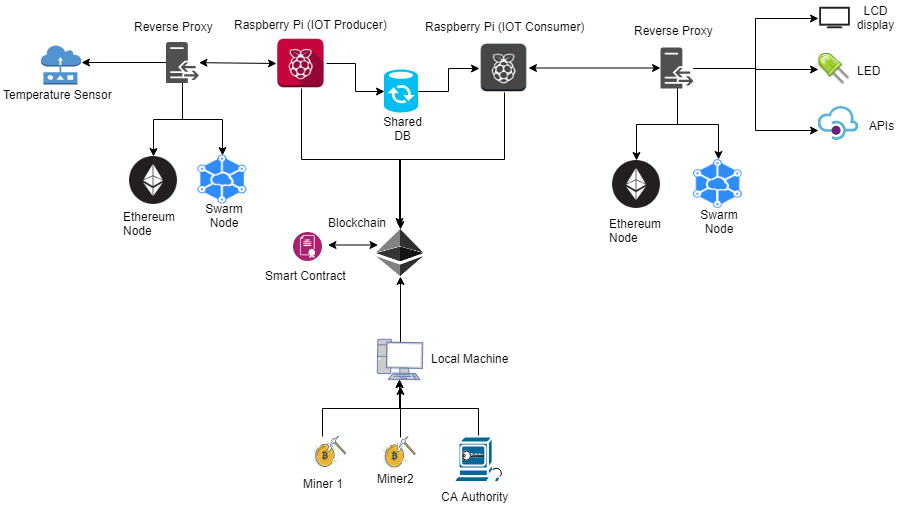
\includegraphics[scale=0.7]{images/Final_Implementation.png}
	\caption{Implementation Diagram}
	\label{fig:impldiagram_architechture}
\end{figure}
\section{Proposed System}
<<>>

\subsection{High-level Design} \label{ss:construct_architecture}
Below is a high-level design to build a private Ethereum network with a raspberry pi generating and saving IOT data from sensors into the blockchain and another raspberry pi retrieving this data and controlling the led attached to it. Another machine serves as the miner node for this network.



\subsection{Node Selection Rule} {
	This section describes how our proposed algorithm chooses our nodes. The node with highest TWU is traversed first. From the Figure \ref{fig:htwui_tree_structure}, the highest TWU item, $Item B$, is traversed and then next item $Item E$ is traversed along with its child nodes. The case is same when traversing inside the child of child nodes. For example, the child nodes of $Item A$ are $Item E$ and $Item B$. The node with $Item B$ is traversed first and then $Item E$ is traversed. Therefore, some of the itemsets formed by traversing the tree are as  $\{B\}, \{E\}, \{E,B\}, \{A\},\{A,B\}, \{A,E\}, \{A,E,B\}$
}

\subsection{Construction of Sub-tree of Itemsets} \label{ss:sub-tree-itemsets}
For the construction of sub-tree of itemsets, a recursive approach is used in which traversing of node starts from the node with higher TWU itemset and the next subsequent node is taken and traversed. It utilizes depth-first search strategy to traverse every node.

Different computation undergoes in the algorithm as shown in Algorithm \ref{alg:build-sub-tree} which includes the computation of projected database, checking the pruning table to prune the transactions, calculation of utility of an itemset, calculation of sub-tree utilities, local utilities and transaction weighted utilities for all its following items, next child nodes of a current itemset and follower nodes of the child node is computed and the insertion of an itemset to pruning table is also carried out in this process.

 {\SetAlgoNoLine
 	\begin{algorithm}[h]
 		\SetKwInOut{Input}{Input}
 		\Input{Transactional Database $D$, ThresholdRatio $\delta$, Total Utility $TU$}
 		\Fn {constructSubTree($\gamma$, $D$, nextNodes($\gamma$), followerItems($\gamma$), $\delta$, TU)}{
 			\For{each item $i_j$ in $nextNodes(\gamma)$}{
 				$\rho \gets \gamma \cup \{i_j\}$\;
 				\While{scan each $T_j$ in $D$}{
 					\uIf {checkPruningTable($T_j$)}{
 						continue from while loop\;}
 					Compute ${\rho}D$\;
 					Calculate $u(\rho)$\;
 				}
 				\uIf{$u(\rho) \ge \delta \times TU$} {$HUIs \gets \rho$\;}
 				Calculate $subU(\rho, x), locU(\rho, x)$ and $TWU(\rho, x)$ for all the items $i_j$ in $followerItems(\gamma)$ by scanning ${\rho}D$\;
 				$nextNodes(\rho) = \{x \in followerItems(\gamma)|subU(\rho, x)\ge \delta \times TU\}$\;
 				$followerItems(\rho) = \{x \in followerItems(\gamma)|locU(\rho, x) \ge \delta \times TU \}$\;
 				\While{scan each item $i_k$ in $followerItems(\gamma)$} {
	 			$i_s \gets \rho \cup i_k$\;
 				\uIf{$TWU(i_s) < \delta \times TU$}{
 					$insertToPruningTable(i_s)$\;}
 				}
 				$constructSubTree(\rho, \rho{D}, nextnodes(\rho), followerItems(\rho), \delta, TU)$\;
 			}
 		}
 		\caption{Build Sub-tree to determine Itemsets}
 		\label{alg:build-sub-tree}
 	\end{algorithm}
 }

\subsection{Pruning Strategies}
In our proposed algorithm, the concept of a pruning hash table is implemented. The detail of the proposed pruning hash table is explained in detail in Transaction Pruning Strategy section below. We also use different utility bounds such as sub-tree utility, local utility and transaction weighted utility to prune the branches.


\subsubsection{Transaction Pruning Strategy}
The proposed algorithm uses a transaction pruning rule to avoid the transactions which contain the itemsets in the pruning hash table to generate the projected transaction ${\rho}D$.

A hash table is implemented to insert itemsets that are to be pruned. The hash table stores the itemsets with low-utility value. While traversing the different nodes, the itemset is inserted into the pruning hash table if the current itemset has transaction weighted utility lower than the threshold value. For example, if an itemset $\{A,B,C\}$ is to be inserted into the pruning table, our proposed algorithm first checks whether there is already a superset of that itemset in the hash table. If pruning hash table does not contain any superset, it then stores an $Item A$ in the map with key as $A$ and $null$ as value. Then, another map with $Item B$ will be inserted as the value in $A$ and so on until all the items are stored in the pruning hash table.
The algorithm to check whether the superset of an itemset is present or not is shown in Algorithm \ref{alg:transaction_pruning} and to insert an itemset in the pruning hash table is shown in Algorithm \ref{alg:insertPtable}.

{\SetAlgoNoLine
	\begin{algorithm}
		\SetKwInOut{Input}{Input}
		\Input{Pruning Hash Table $pTable$, transaction $T_j$}
		\Fn {checkPruningTable($T_j$)} {
			$pr \gets pTable$\;
			\uIf{$pTable.size() > 0$} {
				\For{each item $i_k \in T_j$}{
					//check item in pruning table\newline
					\uIf{$i_k$ not in pr}{return false\;}
					$pr \gets pr(i_k)$\;
					\uIf{pr is null}{return true\;}
				}
			}
			return false\;
		}
		\caption{Checking in Pruning Hash Table for Transaction Pruning}
		\label{alg:transaction_pruning}
	\end{algorithm}
}

{\SetAlgoNoLine
	\begin{algorithm}
		\SetKwInOut{Input}{Input}
		\Input{Itemset $itemset$, Maximum limit of pruning table $\phi$}
		\Fn {insertIntoPruningTable($itemset$)} {
			\uIf{$checkPruningTable(itemset)\;is\;null$} {
				\uIf{$pTable.size() < \phi$} {
						Insert into pruning table recursively;
						
						pTablesize++;
					
					return true;
					
				}
			}
			return false;
		}
		\caption{Insertion in Pruning Hash Table}
		\label{alg:insertPtable}
	\end{algorithm}
}


\subsubsection{Utility Based Pruning}
Our proposed algorithm uses utility based pruning to prune the branches with itemsets that are not feasible. Utility based pruning includes sub-tree utility, local utility and transaction weighted utility. The transaction weighted utility of an itemset prunes the itemset that is less than the minimum threshold by inserting into the pruning hash table which is used for reducing the search space. During the generation of projected transaction, while traversing on each node, calculation of sub-tree utility and local utility are done for each of the possible follower items of that node. If any of the possible follower items have sub-tree utility less than the minimum threshold, then that item cannot be the next possible node but still has a chance to be the follower item for the next nodes of the current itemset. If those possible follower items of a node have local utility less than the minimum threshold, it cannot be the next node as well as a follower item for that node. For example, let us consider a node as $Item A$ and suppose, there are 3 possible follower items $Item B, Item C$ and $Item D$. The sub-tree utility is calculated for all its follower items $B, C$ and $D$ and if B has sub-tree utility  greater than threshold value and $C$ and $D$ have sub-tree utility value less than threshold then, $Item B$ is the next node as well as the follower item for $Item A$ but the local utility is calculated for $Item C$ and $Item D$ and suppose if $Item C$ has local utility greater than threshold value and $Item D$ has local utility less than threshold, then $Item C$ can be the follower item of node $Item A$. Therefore, next node of $Item A$ is $\{B\}$ and follower items is $\{B,C\}$.

\subsection{Detailed Algorithm (HUI-PR)}
Our detailed algorithm is shown in Algorithm \ref{alg:find_huis}. Our algorithm starts with reading the transactional database ($TD$) and threshold ratio ($\delta$). The total utility ($TU$), transaction weighted utility ($TWU$) of items and local utility ($locU$) of all the items of a database is computed by scanning the whole transactional database. Total utility of an database, transaction weighted utility of items and local utility of items are calculated as defined in Equation \ref{eq:totalUtil}, \ref{eq:tranUtil} and \ref{eq:local_utility}. 1-HTWUIs are calculated based on the transaction weighted utility obtained as described in Section \ref{ss:construct_1htuwis}. The follower items are 1-HTWUIs for the initial node and these items are sorted in increasing order in total ordering ($\rightarrow$) as described in Definition \ref{def:total_ordering}. From the list of 1-HTWUIs, those itemsets with transaction weighted utility values less than the threshold are known as unpromising items. Moreover, those unpromising items are removed from the transactions of the whole transactional database. After removing the unpromising items from the database, if there are empty transactions created, then those transactions are removed. The items of each transaction in the transactional database are sorted based on the total ordering. Calculation of sub-tree utility for each followerItems is done by scanning the whole database and based on the sub-tree utility values, next nodes of the initial root node are defined where the items must have sub-tree utility greater than the threshold. Sub-tree is constructed recursively with taking the parameters as the transactional database, nextNodes, followerItems, thresholdRatio and total utility. The algorithm to find the sub-tree of itemsets is defined in detail in Section \ref{ss:sub-tree-itemsets}.

{\SetAlgoNoLine
	\begin{algorithm}
		\SetKwInOut{Input}{Input}
		\SetKwInOut{Output}{Output}
		
		\Input{Transactional Database $TD$, ThresholdRatio $\delta$}
		\Output{High Utility Itemsets $HUIs$}
		Initial itemset, $\gamma$ = $\phi$\;
		Calculate Total Utility $TU$, $TWU(\gamma, i_j)$ and local utility $locU(\gamma, i_j)$ for all $i_j \in I$ by scanning whole database $TD$\;
		Compute 1-HTWUIs itemsets, \newline $followerItems(\gamma) = \{i_j | i_j \in I \cap TWU(\gamma, i_j) \ge \delta \times TU\}$ \newline
		Sort the items in $followerItems(\gamma)$ in total ordering ($\rightarrow$)\;
		Remove the unpromising items $j$ from the transactions $T_j$\;
		Remove the empty transaction after removing unpromising items\;
		Sort the items in each transaction in total ordering ($\rightarrow$)\;
		Calculate sub-tree utility $subU(\gamma, i_j)$ for all $i_j \in followerItems(\gamma)$ by scanning database $TD$\;
		Compute next nodes to visit in reverse order, \newline $nextNodes(\gamma) = \{i_j|i_j \in reverse(followerItems(\gamma)) \cap subU(\gamma, i_j) \ge \delta \times TU \}$\;
		$constructSubTree(\gamma, TD, nextNodes(\gamma), followerItems(\gamma), \delta, TU)$\;
		\caption{Algorithm to find HUIs}       	
		\label{alg:find_huis}
	\end{algorithm}
}

\section{Method II - Distributed EFIM}
This section describes our proposed algorithm EFIM Parallel (EFIM-Par) to find high utility itemsets with parallel computing using Apache Spark. This algorithm is the parallel (distributed) implementation of the algorithm EFIM \cite{Zida2015}. This section comprises of generating 1-HTWUIs, generating revised transactions, finding the sub-tree utility and the local utility, assigning the sub-tree to worker nodes, node data generation, mining high utility itemsets by individual worker nodes and explanation of the overall flow of EFIM Parallel algorithm.

\subsection{Generating 1-HTWUIs with their corresponding TWU} \label{ss:generate_1htwuis}
The Transactional Database $(TD)$ is scanned to find out the 1-HTWUIs of items along with their transaction weighted utility. First of all, the transactional database is divided into different blocks which are computed by different worker nodes using $flatMap$ operation. The result obtained from worker nodes are reduced using $reduceByKey$ operation to get the itemTWU of items which contain items with their corresponding TWU.

\subsection{Generating Revised Transactional Database} \label{ss:generate-revised-transactions}
In this process, the Transactional Database $(TD)$ is mapped to generate the revised transactional database using map operation. Firstly, $TD$ is split into different blocks to distribute among worker nodes in which pruning of unpromising items are done, and then the transaction is sorted in the ascending order of the transaction weighted values of items. Besides pruning of unpromising items and sorting, there is a removal of empty transactions by using filter operation. The generated revised transactions use the functionality provided by Spark to persist the RDD so that it can be used again later. It is used later to find out the sub-tree utility of items and assignment of items to worker nodes which will be described in the later sections.

{\SetAlgoNoLine
	\begin{algorithm}
		\SetKwInOut{Input}{Input}
		\SetKwInOut{Output}{Output}
		
		\Input{Transactional Database $TD$, ThresholdRatio $\delta$, Total Utility $TU$}
		\Output{Revised Transactional Database}
		
		\Fn{map()}{
			\For{k = 0 to len(TD)-1}{
				// Removing unpromising items from the transaction
				$TD_k = \sum_{j = 0}^{len(TD_k)-1}\{i_j | i_j \in TD_k \cap TWU(i_j) \geq \delta \times TU \}$;
				
				// Sort items in transaction in total ordering
				
				$SortItems(TD_k)$;
				
				\If{$len(TD_k)$ == 0}{Remove $TD_k$;}
			}
		}
		\caption{Revised Transactional Database Generation}           
		\label{alg:revised_transaction_generation}
	\end{algorithm}
}

\subsection{Finding Local Utility and Sub-tree Utility of 1-HTWUIs}
There are two utilities in this proposed algorithm which prunes the unnecessary visitation of the nodes. It reduces the search space significantly. It needs to be calculated in the first level of the tree in order to compute the next nodes of each item and the follower nodes of those items. The local utility is calculated as shown in Equation \ref{eq:local_utility}. For the initial case, it is same as transaction weighted utility, therefore, it uses TWU of 1-HTWUIs as described in Section \ref{ss:generate_1htwuis}. Another utility is the sub-tree utility which is calculated as shown in the Equation \ref{eq:sub_utility}. It scans the revised transaction to generate the sub-tree utility for each item of 1-HTWUIs. It uses flatMap and Reduce operations to get the sub-tree utility values for each item.

\subsection{Sub-tree Assignment to Worker Nodes} \label{ss:sub-tree-to-workernodes}
The proposed algorithm uses grouping strategy to assign the $itemsToExplore$ and their respective sub-trees to the worker nodes. The $itemsToExplore$ is computed by using the Equation \ref{eq:itemsToExplore}. Grouping of 1-HTWUIs is as shown in the Algorithm \ref{alg:workernode_assignment}. This grouping approach helps to divide our tasks among the worker nodes to be executed in distributed environment properly. The grouping is done based on the number of items to explore. Items to explore is defined in Equation \ref{eq:itemsToKeep}.

Referring to the example in Table \ref{table:quantitative_db} and \ref{table:profit_table}, we have 7 items in which there are 6 1-HTWUI items. From the definition of \ref{def:itemsToExplore}, we have $D, F, C, A, E, B$ as items to explore. Let us suppose we have 3 worker nodes as $Node\ 1$, $Node\ 2$ and $Node\ 3$. According to the Algorithm \ref{alg:workernode_assignment}, the worker nodes are assigned as $D \rightarrow Node\ 1$, $F \rightarrow Node\ 2$, $C \rightarrow Node\ 3$, $A \rightarrow Node\ 3$, $E \rightarrow Node\ 2$ and $B \rightarrow Node\ 1$. The worker nodes are assigned to the sub-tree nodes along with their respective node data which is described in Section \ref{ss:generate_nodedata}.
{\SetAlgoNoLine
	\begin{algorithm}
		\SetKwInOut{Input}{Input}
		\SetKwInOut{Output}{Output}
		
		\Input{Number of worker nodes $N$, Follower nodes $itemsToExplore$}
		\Output{Hashmap($nodeId$, $itemsToExplore$) $workerNodeMap$}
		
		\Fn{grouping()}{
			$workerNodeMap \gets map()$;
			
			$nodeId \gets 1$;
			
			$incr \gets 1$;
			
			$flag \gets false$;
			
			\For{i in itemsToExplore}{
				$workerNodeMap[i] \gets nodeId$;
				
				$nodeId \gets nodeId + 1$;
				
				\If{$(nodeId == 0\ ||\ nodeId == N-1)$}{
					\eIf{$(flag == false)$}{
						$incr \gets 0$;
						
						$flag \gets true$;
					} {
						\eIf{$(nodeId == 0)$}{$incr \gets 1$;}{$incr \gets -1$;}
						$flag \gets false$;
					}
				}
			}
			return $workerNodeMap$;
		}
		\caption{Assignment of Sub-tree to Worker Nodes}           
		\label{alg:workernode_assignment}
	\end{algorithm}
}

\newpage
\subsection{Node Data Generation} \label{ss:generate_nodedata}
Each worker node is assigned with a sub-tree which needs to be traversed. Each node traversal indicates the candidate generation which is needed to generate projected transaction at each node. Therefore, each worker node gets the refined transactions including the items it needs to visit which is computed using flatMap operation. Algorithm \ref{alg:nodedata_generation} shows the steps to generate the node data for the specific items assigned to the worker nodes. Each transaction is checked by the binary search to find the item assigned to worker node is present or not. If items assigned are not in the transaction, then that transaction is not added to the nodeMap. After scanning all the nodes, nodeMap is grouped by a key which is then used to mine high utility itemsets which are explained in Section \ref{ss:minehuis} later.

{\SetAlgoNoLine
	\begin{algorithm}
		\SetKwInOut{Input}{Input}
		\SetKwInOut{Output}{Output}
		
		\Input{Revised Transactions $T$, $workerNodeMap$}
		\Output{Hashmap($nodeId$, $T_r$) $nodeMap$}
		
		\Fn{flatMap}{
			$nodeMap = map();$
			
			\For{$i \gets 0\ to\ len(T)-1$ }{
				
				\For{$(nodeId, item) \gets workerNodeMap$}{
					
					$check = binarySearchIterative(T.itemset, item)$;
					
					\If{$check$ == true}{
						$nodeMap \gets (nodeId, T_i)$;
					}
				}
			}
			return $nodeMap$;
		}
		\Fn{binarySearchIterative(list, target)}{
			$left \gets 0$;
			$right \gets len(list) - 1$;
			
			\While{$(left \leq right)$} {
				$mid = left + (right - left)\ /\ 2$;
				
				\uIf {(list(mid) == target)}
				{
					return $true$;
				} \uElseIf{$list(mid) \ge target$} {
					$right = mid - 1$;
				} \Else {
					$left = mid + 1$;
				}
			}
			return $false$;
		}
		\caption{Node Data Generation}           
		\label{alg:nodedata_generation}
	\end{algorithm}
}

\newpage
\subsection{Mining High Utility Itemsets} \label{ss:minehuis}
This section describes the mining of high utility itemsets that are computed by worker nodes using generated Node data. The detailed algorithm is shown in Algorithm \ref{alg:mine_huis_distributed}. Each worker processes to compute the high utility itemsets (HUIs) for the assigned sub-tree of items. It uses a recursive algorithm to find HUIs which generates the possible candidate sets assigned to them. Let us consider the example from the Figure \ref{fig:htwui_tree_structure} in which each item of 1st level is assigned to one worker node. Let us assume that there are 3 worker nodes, then we know from the previous Section \ref{ss:sub-tree-to-workernodes}, $ItemD$ is assigned to $Node 1$. All the possible candidate sets for $ItemD$ are processed by $Node1$. Similarly, for the $ItemF$, possible candidate sets are processed by $Node2$ and so on.

{\SetAlgoNoLine
	\begin{algorithm}
		\SetKwInOut{Input}{Input}
		\SetKwInOut{Output}{Output}
		\Input{Database $d$, ThresholdRatio $\delta$, Total Utility $TU$, $nodeMap$, $nodeId$}
		\Output{High Utility Itemsets $HUIs$}
		\Fn {mineHUIs($\gamma$, d, itemsToExplore($\gamma$), itemsToKeep($\gamma$), $\delta$, TU, $flagFirst = true$)}{
			\For{each item $i_j$ in $itemsToExplore(\gamma)$}{
				\If{$(flag \ne true\ ||\ nodeId == nodeMap(i))$}{
					$\rho \gets \gamma \cup \{i_j\}$\;
					\While{scan each $T_j$ in ${\gamma}D$}{
						Compute ${\rho}D$\;
						Calculate $u(\rho)$\;
					}
					\uIf{$u(\rho) \ge \delta \times TU$} {$HUIs \gets \rho$\;}
					Calculate $subU(\rho, x)$ and $locU(\rho, x)$ for all the items $i_j$ in $itemsToKeep(\gamma)$ by scanning ${\gamma}D$\;
					$itemsToExplore(\rho) = \{x \in itemsToKeep(\gamma)|subU(\rho, x)\ge \delta \times TU\}$\;
					$itemsToKeep(\rho) = \{x \in itemsToKeep(\gamma)|locU(\rho, x) \ge \delta \times TU \}$\;
					$mineHUIs(\rho, d, itemsToExplore(\rho),$$itemsToKeep(\rho), \delta, TU, false)$\;
				}
			}
		}
		\caption{Mining HUIs in Parallel}
		\label{alg:mine_huis_distributed}
	\end{algorithm}
}

\newpage
\subsection{Overall Flow of EFIM Parallel Algorithm}
The overall flow diagram of EFIM Parallel Algorithm is shown in Figure \ref{fig:flowdiagram_efimpar}. It starts with reading of dataset from the file which is split into different blocks to be distributed among the worker nodes. The worker nodes work on the block of the file using $flatMap$ operation to generate the key-value pairs of items and its corresponding TWU which is then combined using $ReduceByKey$ operation to get the final $itemTWU$. The generation of 1-HTWUIs was explained in detail in the previous Section \ref{ss:generate_1htwuis}. The split dataset is also used to find the total utility of the transactional database to find the threshold value. This threshold value is used to find the $itemsToKeep$ by filtering out the items in 1-HTWUIs having TWU values less than the threshold value. Only those items remaining in the $itemsToKeep$ are kept in the transactions of the database. Therefore, other items not in $itemsToKeep$ known as unpromising items, are removed from the transactions, sort the items in a transaction in the total ordering and removal of empty transactions are done to get the sorted revised transactions which were described in detail in Section \ref{ss:generate-revised-transactions}. In the next step, the sorted revised transactions are used to find the $utilityBinSU$ for each items by using $flatMap$ and $ReduceByKey$ operations. The $utilityBinSU$ contains sub-tree utility for all the items of $itemsToKeep$. The $utilityBinLU$ contains local utility for all the items which is same as the $itemTWU$. Using the $utilityBinSU$, the list containing all the items for $itemsToExplore$ is created. A sub-tree is created from the items in $itemsToExplore$.

Assignment of items of $itemsToExplore$ is done using the grouping mechanism as described in detail in Section \ref{ss:sub-tree-to-workernodes}. In this process, the worker node identifies the sub-tree it needs to generate. Each worker node processes to filter the transactions to produce the Node Data. Using these node data, each worker node mines the high utility itemsets forming sub-trees to generate the candidate sets. In the mining process, the nodes are pruned based on the sub-tree utility and the local utility as given in Equation \ref{eq:sub_utility} and Equation \ref{eq:local_utility} respectively. Finally, the results obtained from the worker nodes are combined to give the aggregated high utility itemsets.

\begin{figure}
	\centering
	\includegraphics[scale=0.7]{Flowdiagram-distributed}
	\caption{Overall Flow Diagram of EFIM Parallel Algorithm}
	\label{fig:flowdiagram_efimpar}
\end{figure}

%To main things in \LaTeX should be labelled: Figures and Tables.
%
%\section{Figures}
%
%The file {\tt unlv\_macros.tex} contains a number of spiffy macros to
%make figures for you. For example, Fig.~\ref{fig:fancy} is generated
%by the
%command:\\ \verb+\DoFigure{radiusball}{0.5}{This is a fancy picture}{fig:fancy}+. The
%command takes in 4 arguments: the pdf file's name (without .pdf), the
%scaling factor, the caption and the label name (which you can later
%use to refer to the figure's number.)
%
%\DoFigure{radiusball}{0.5}{This is a fancy picture}{fig:fancy}
%
%\newpage 
%\noindent
%We could have built the same directly (see Fig.~\ref{fig:fancy2}) like this:\\
%
%\noindent
%\verb+\begin{figure}[htb!]+\\
%\verb+\begin{center}+\\
%\verb+\includegraphics[scale=0.5]{radiusball}+\\
%\verb+\caption{This is a fancy picture again.}\label{fig:fancy2}+\\
%\verb+\end{center}+\\
%\verb+\end{figure}}+\\
%
%
%\begin{figure}[htb!]
%\begin{center}
%\includegraphics[scale=0.5]{radiusball}
%\caption{This is a fancy picture again.}\label{fig:fancy2}
%\end{center}
%\end{figure}
%
%The macro package also contains macros for double pictures:
%
%\DoBiFigure{radiusball}{radiusball}{0.4}{A shared caption for the pictures.}{fig:double}
%
%or for double pictures with separate captions:
%
%\DoDiFigure{radiusball}{0.4}{A caption for the left pictures.}{fig:di1}{radiusball}{0.4}{A caption for the right pictures.}{fig:di2}
%
%\section{Tables}
%
%A table is most easily made with the {\tt tabular} environment. This environment can 
%produce {\it very} fancy tables, so you might need to go look it up on the web.
%
%\begin{table}[!htb]
%\begin{center}
%\begin{tabular}{||c|l|r||} \hline
%Column 1 & Column 2 & Column 3 \\ \hline\hline
%Foo & 1\" & 2.54cm\\
%Bar & 2\" & 6.08cm\\ \hline
%Baz & \multicolumn{2}{|c||}{Who knows?} \\ \hline
%\end{tabular}
%\caption{A table!}\label{tab:atable}
%\end{center}
%\end{table}

\chapter{Experimental Results}
\label{chapter:experiment_results}
The experiments were performed for our Method I with our proposed algorithm (HUI-PR) and EFIM algorithm \cite{Zida2015} to find high utility itemsets on 16GB main memory in Intel Xeon(R) CPU E5-1607 0 @ 3.00 GHz x 4 on an Ubuntu 16.04 Linux Operating system. The language used to write these algorithms was Oracle Java 1.8. 

For the Method II, the experiments were performed on Spark clusters with Master and all Slave nodes with 16GB main memory and Intel Xeon(R) CPU E5-2695 v4 @ 2.10 GHz x 4 with an Ubuntu 16.04 Linux Operating system. The language used to write the spark application was Scala version 2.12.1 with Spark framework version 2.0.2 to run an experiment for our proposed algorithm EFIM-Par and PHUI-Miner \cite{Chen2016}.

\section{Datasets}
The experiments were performed on multiple real-world datasets \cite{miningdataset2012, SPMFDatasets}. For the method I, our experiments were conducted on smaller datasets such as Chess, Connect and Retail. For the method II, our experiments were conducted on relatively large datasets such as Connect20x, Chess30x, BMS4x, Mushroom20x. For large datasets, the small datasets such as Connect, Chess, BMS and Mushroom were multiplied to get the larger dataset. The characteristics of the datasets are shown in the Table \ref{dataset_table} where $\#|D|$, $\#|I|$, $AvgLen$, $MaxLen$, $Type$ and $Scale$ represent the total number of transactions, the number of distinct items, the average size of a transaction, maximum size of a transaction, type of dataset and size of dataset respectively. For each threshold ratio of a dataset, the experimental results were executed 10 times and the average was taken.

\begin{table}[!htbp]
	\renewcommand{\arraystretch}{1.3}
	\caption{Datasets Characteristics}
	\label{dataset_table}
	\centering
	\begin{tabular}{|c||c|c|c|c|c|c|}
		\hline
		\bfseries Dataset & \bfseries $\#|D|$ & \bfseries $\#|I|$ & \bfseries AvgLen & \bfseries MaxLen & \bfseries Type & \bfseries Scale\\
		\hline\hline
		$chess$ & 3196 & 76 & 37 & 37 & dense & Small\\ \hline
		$connect$ & 67557 & 129 & 43 & 43 & dense & Small\\ \hline
		$retail$ & 88162 & 16470 & 10 & 76 & sparse & Medium \\ \hline
		$connect2x$ & 135114 & 129 & 43 & 43 & dense & Large\\ \hline
		$chess30x$ & 95880 & 76 & 37 & 37 & dense & Large\\ \hline
		$BMS4x$ & 238408 & 497 & 3 & 267 & sparse & Large \\ \hline
		$Mushroom20x$ & 162400 & 119 & 23 & 23 & dense & Large\\ \hline
	\end{tabular}
\end{table}

\section{HUI-PR vs EFIM}
Our proposed HUI-PR was compared with EFIM \cite{Zida2015} with comparisons on the computational time, the number of high utility itemsets (HUIs) found and the number of Candidate Sets generated. These algorithms were performed on the smaller datasets.

\subsection{Comparison of Computational Time}
In this section, we compared our algorithm (HUI-PR) with the EFIM algorithm \cite{Zida2015} with the real datasets (Connect, Chess, Retail). Experiments were conducted to show the effectiveness of our algorithm with the real datasets and the approach that was taken to improve the performance of an experiment. The pruning rule proposed in our algorithm HUI-PR helps to improve computational time significantly for the datasets with a large number of transactions. The proposed algorithm generates the projected transaction which reduces the number of transactions in each level. It not only reduces the number of transactions based on utility calculations but it also uses the pruning hash table to eliminate the transactions in which the itemsets in the pruning table might be a subset of items in a transaction. Therefore, it helps to check whether the items in a transaction are a superset or not in very quick time.

From the Figure \ref{fig:graph-comparison}, we see that HUI-PR can perform better than the EFIM algorithm. From the Figure \ref{fig:graph-connect}, for the ``Connect" dataset, the threshold ratio was set from 28.90\% to 29.70\% as shown. When the threshold ratio was 28.90\%, our algorithm HUI-PR took 1830.87 seconds while the EFIM algorithm took 1927.95 seconds. The proposed algorithms showed significant improvement in Figure \ref{fig:graph-retail} on threshold ratio 0.03\%, the running time for HUI-PR was 5718.36 seconds while for EFIM algorithm, the running time was 7370.33 seconds.

We also conducted our experiment against the other state-of-the-art algorithms: HUI-Miner \cite{Liu2012}, HUP-Miner \cite{Krishnamoorthy2015}, FHM \cite{Fournier-Viger2014}, FHM+ \cite{Fournier-Viger2016}, d\textsuperscript{2}HUP \cite{Krishnamoorthy2015, Liu2012}. Our algorithm HUI-PR performs better than these state-of-the-art algorithms as shown in Figure \ref{fig:graph-multiple-comparison}. For the ``Connect" dataset, our algorithm performed better by more than 100 times than HUI-Miner, HUP-Miner and FHM algorithms while it performed better by almost 50 times than d\textsuperscript{2}HUP. Similarly, for the ``Chess" dataset, HUI-PR performed better by 20 times than HUI-Miner, HUP-Miner and FHM algorithms while it performed better than 7 times than d\textsuperscript{2}HUP. Since the time performed by FHM+ was significantly higher when it was executed with parameter $MaxLength=15$ for the ``Chess" dataset and $MaxLength=21$ for the ``Connect" dataset. Therefore, it is not shown in the graph.

\begin{figure}
	\begin{subfigure}{\textwidth}
		\centering 
		\includegraphics[scale=0.5]{RuntimeConnect-HUIPRvEFIM}
		\subcaption{Connect Dataset}
		\label{fig:graph-connect}
	\end{subfigure}    
	\begin{subfigure}{\textwidth}
		\centering
		\includegraphics[scale=0.5]{RuntimeChess-HUIPRvEFIM}
		\subcaption{Chess Dataset}
		\label{fig:graph-chess}
	\end{subfigure}
	\begin{subfigure}{\textwidth}
		\centering 
		\includegraphics[scale=0.5]{RuntimeRetail-HUIPRvEFIM}
		\subcaption{Retail Dataset}
		\label{fig:graph-retail}
	\end{subfigure}
	\caption{Comparison of computational time between HUI-PR and EFIM w.r.t. variants of minimum threshold for different datasets}
	\label{fig:graph-comparison}
\end{figure}
\begin{figure}
	\centering 
	\begin{subfigure}[b]{\textwidth}
		\centering
		 \includegraphics[scale=0.7]{RuntimeConnect-HUIPRvAll}
		\subcaption{Connect Dataset}
		\label{fig:graph-connect-comparison}
		\bigskip
	\end{subfigure}
	\begin{subfigure}[b]{\textwidth}
		\centering
		\includegraphics[scale=0.7]{RuntimeChess-HUIPRvAll}
		\subcaption{Chess Dataset}
		\label{fig:graph-chess-comparison}
	\end{subfigure}
	\caption{Comparison of computational time with state-of-the-art algorithms w.r.t. variants of minimum threshold}
	\label{fig:graph-multiple-comparison}
\end{figure}


\subsection{Comparison of HUIs}
From the experiments conducted on the real-world datasets (Connect, Chess and Retail), the number of HUIs found by both the experiments are same. We recorded the number of HUIs found for the range of threshold ratio for different datasets which are shown in Table \ref{table:result_huis}. For the ``Connect" database, we got 81 HUIs for 28.90\% and 4 HUIs for 29.70\%. Similarly, for the ``Chess" dataset, we got 342 HUIs for 24.00\% and 16 HUIs for 26.00\% threshold ratio. From the results obtained, we can verify that all the high utility itemsets have been found from our proposed algorithm HUI-PR.


\begin{table}
	\renewcommand{\arraystretch}{1.3}
	\caption{Total Number of HUIs found in HUI-PR and EFIM}
	\label{table:result_huis}
	\centering
	\begin{tabular}{|c||c|c|}
		\hline
		\bfseries Dataset & \bfseries ThresholdRatio $\delta$ & \bfseries \# of HUIs\\
		\hline\hline
		$Connect$ & 28.90\% & 81\\ \hline
		$Connect$ & 29.10\% & 40\\ \hline
		$Connect$ & 29.30\% & 20\\ \hline
		$Connect$ & 29.50\% & 8\\ \hline
		$Connect$ & 29.70\% & 4\\ \hline \hline
		
		$Chess$ & 24.00\% & 342\\ \hline
		$Chess$ & 24.50\% & 177\\ \hline
		$Chess$ & 25.00\% & 98\\ \hline
		$Chess$ & 25.50\% & 41\\ \hline
		$Chess$ & 26.00\% & 16\\ \hline \hline
		
		$Retail$ & 0.30\% & 92\\ \hline
		$Retail$ & 0.40\% & 58\\ \hline
		$Retail$ & 0.50\% & 41\\ \hline
		$Retail$ & 0.60\% & 30\\ \hline
		
	\end{tabular}
\end{table}

\begin{table}
	\renewcommand{\arraystretch}{1.3}
	\caption{Total Number of Transactions Pruned in HUI-PR}
	\label{result_transactions_pruned}
	\centering
	\begin{tabular}{|c||c|c|}
		\hline
		\bfseries Dataset & \bfseries ThresholdRatio $\delta$ & \bfseries \# Transactions Pruned\\        \hline\hline
		
		$Connect$ & 28.90\% & 556831\\ \hline
		$Connect$ & 29.10\% & 550630\\ \hline
		$Connect$ & 29.30\% & 550630\\ \hline
		$Connect$ & 29.50\% & 550630\\ \hline
		$Connect$ & 29.70\% & 550630\\ \hline \hline
		
		$Chess$ & 24.00\% & 24878\\ \hline
		$Chess$ & 24.50\% & 30779\\ \hline
		$Chess$ & 25.00\% & 27829\\ \hline
		$Chess$ & 25.50\% & 26265\\ \hline
		$Chess$ & 26.00\% & 26304\\ \hline \hline
		
		$Retail$ & 0.30\% & 670018\\ \hline
		$Retail$ & 0.40\% & 245342\\ \hline
		$Retail$ & 0.50\% & 117453\\ \hline
		$Retail$ & 0.60\% & 61939\\ \hline
		
	\end{tabular}
\end{table}


\subsection{Comparison of Candidate Sets}
From the Figure \ref{fig:comparison-candidatesets-efim}, we compared the candidate sets obtained from HUI-PR and EFIM algorithms. The candidate sets generated in HUI-PR are lower in number than that in EFIM algorithm. The candidate sets are minimized in the HUI-PR using transaction pruning strategies with pruning hash table and utility based pruning. For the ``Connect" dataset for threshold ratio 28.90\%, HUI-PR generated 3007 candidate sets while the EFIM algorithm generates 3132 candidate sets. HUI-PR could generate fewer candidate sets in the ``Chess" dataset. For 24.00\% threshold ratio, HUI-PR generated 2933 candidate itemsets while EFIM generated 2965 number of candidate itemsets. We also compared the candidate sets obtained from state-of-the-art algorithms: HUIMiner, FHM and FHM+ as shown in Figure \ref{fig:graph-candidatesets-comparison}. The number of candidate sets generated by our algorithm HUI-PR is 8 times less than HUIMiner and FHM for the ``Chess" dataset while HUI-PR generates 10 times less than HUIMiner and FHM for the ``Connect" dataset.

\begin{figure}
	\centering
	\begin{subfigure}[b]{\textwidth}
		\centering
		\includegraphics[scale=0.5]{CandidateSetsConnect-EFIM}
		\subcaption{Connect Dataset}\label{fig:connect-candidatesets}
	\end{subfigure}
	\begin{subfigure}[b]{\textwidth}
		\centering
		\includegraphics[scale=0.5]{CandidateSetsChess-EFIM}
		\subcaption{Chess Dataset}\label{fig:chess-candidatesets}
	\end{subfigure}
	\begin{subfigure}[b]{\textwidth}
		\centering
		\includegraphics[scale=0.5]{CandidateSetsRetail-EFIM}
		\subcaption{Retail Dataset}\label{fig:retail-candidatesets}
	\end{subfigure}
	\caption{Comparison of candidate sets between HUI-PR and EFIM w.r.t. variants of minimum threshold}
	\label{fig:comparison-candidatesets-efim}
\end{figure}

\begin{figure}
	\centering
	\begin{subfigure}[b]{\textwidth}
		\centering
		\includegraphics[scale=0.7]{CandidateSetsConnect-HUIPRvsAll}
		\subcaption{Connect Dataset}
		\label{fig:graph-connect-candidatesets}
		\bigskip
	\end{subfigure}
	\begin{subfigure}[b]{\textwidth}
		\centering
		\includegraphics[scale=0.7]{CandidateSetsChess-HUIPRvsAll}
		\subcaption{Chess Dataset}\label{fig:graph-chess-candidatesets}
	\end{subfigure}
	\caption{Comparison of candidate sets with state-of-the-art algorithms w.r.t. variants of minimum threshold}
	\label{fig:graph-candidatesets-comparison}
\end{figure}

\section{EFIM-Par vs EFIM}
We compared our proposed distributed algorithm Parallel EFIM (EFIM-Par) with Approximate parallel high utility itemset mining (PHUI-Miner) \cite{Chen2016}. The computational time were recorded for the different datasets as shown in the Figure \ref{fig:graph-comparison-distributed}. These algorithms were performed on the larger datasets. Our algorithm were conducted on one master node and ten slave nodes in the Spark Framework.

\subsection{Comparison of Computational Time}
In this section, we ran our experiments on the real-world datasets (Connect, Chess, BMS and Mushroom). However, in order to make the datasets sufficiently large, we multiplied the ``Connect" dataset by a factor of 2, ``Chess" dataset by a factor of 30, ``BMS" dataset by a factor of 4 and ``Mushroom" dataset by a factor of 20. The experiments were conducted on our proposed algorithm EFIM-Par and PHUI-Miner.

From the Figure \ref{fig:graph-connect2x-distributed}, our algorithm EFIM-Par took 76.36 seconds while PHUI-Miner took 161.76 seconds for the threshold ratio 28.90\% for the ``Connect" dataset. Similarly, for the threshold ratio 29.70\%, our EFIM-Par took 64.42 seconds while PHUI-Miner took 113.27 seconds. Our algorithm EFIM-Par was able to perform around 2 times better than PHUI-Miner for the ``Connect" dataset for different threshold ratio taken. From the Figure \ref{fig:graph-chess30x-distributed}, for the ``Chess30x" dataset, our algorithm took 60.77 seconds for the threshold ratio 24.00\% while PHUI-Miner took 79.19 seconds. Similarly, for the threshold ratio 26.00\%, EFIM-Par took 51.97 seconds while PHUI-Miner took 71.03 seconds. Our algorithm performed almost 1.5 times better than PHUI-Miner for the ``Chess30x" dataset. Similarly for the ``BMS4x" dataset, our algorithm performed better for the lower threshold and almost similar for the higher threshold values. Our algorithm performed better than 1.2 times the PHUI-Miner algorithm for ``Mushroom20x" dataset.

\subsection{Comparison of HUIs}
From the Table \ref{table:result-huis-distributed}, we found that our algorithm EFIM-Par found the same number of HUIs as found by PHUI-Miner. Therefore, we can conclude our algorithm is as accurate as PHUI-Miner.

\begin{figure}
	%    \centering
	\begin{subfigure}{\textwidth}
		\centering
		\includegraphics[scale=0.6]{RuntimeConnect2x-Distributed}
		\subcaption{Connect2x Dataset}
		\label{fig:graph-connect2x-distributed} 
		\bigskip
	\end{subfigure}    
	\begin{subfigure}{\textwidth}
		\centering
		\includegraphics[scale=0.6]{RuntimeChess30x-Distributed}
		\subcaption{Chess30x Dataset}
		\label{fig:graph-chess30x-distributed}
	\end{subfigure}
	\caption{Comparison of computational time between EFIM-Par and PHUI-Miner w.r.t. variants of minimum threshold for different datasets}
\end{figure}
\begin{figure} \ContinuedFloat
	\begin{subfigure}{\textwidth}
		\centering
		\includegraphics[scale=0.6]{RuntimeBMS4x-Distributed}
		\subcaption{BMS4x Dataset}
		\label{fig:graph-bms-distributed} 
		\bigskip
	\end{subfigure}
	\begin{subfigure}{\textwidth}
		\centering
		\includegraphics[scale=0.6]{RuntimeMushroom20x-Distributed}
		\subcaption{Mushroom20x Dataset}
		\label{fig:graph-mushroom20x-distributed} 
	\end{subfigure}
	\caption{Comparison of computational time between EFIM-Par and PHUI-Miner w.r.t. variants of minimum threshold for different datasets}
	\label{fig:graph-comparison-distributed}
\end{figure}

\begin{table}
	\renewcommand{\arraystretch}{1.3}
	\caption{Total Number of HUIs found in EFIM-Par and PHUI-Miner}
	\label{table:result-huis-distributed}
	\centering
	\begin{tabular}{|c||c|c|}
		\hline
		\bfseries Dataset & \bfseries ThresholdRatio $\delta$ & \bfseries \# of HUIs\\
		\hline\hline
		$Connect2x$ & 28.90\% & 81\\ \hline
		$Connect2x$ & 29.10\% & 40\\ \hline
		$Connect2x$ & 29.30\% & 20\\ \hline
		$Connect2x$ & 29.50\% & 8\\ \hline
		$Connect2x$ & 29.70\% & 4\\ \hline \hline
		
		$Chess30x$ & 24.00\% & 342\\ \hline
		$Chess30x$ & 24.50\% & 177\\ \hline
		$Chess30x$ & 25.00\% & 98\\ \hline
		$Chess30x$ & 25.50\% & 41\\ \hline
		$Chess30x$ & 26.00\% & 16\\ \hline \hline
		
		$BMS$ & 2.08\% & 7\\ \hline
		$BMS$ & 2.10\% & 7\\ \hline
		$BMS$ & 2.40\% & 5\\ \hline
		$BMS$ & 2.80\% & 3\\ \hline
		$BMS$ & 3.00\% & 2\\ \hline
		
		$Mushroom20x$ & 14.00\% & 67\\ \hline
		$Mushroom20x$ & 14.25\% & 38\\ \hline
		$Mushroom20x$ & 14.50\% & 19\\ \hline
		$Mushroom20x$ & 14.75\% & 10\\ \hline
		$Mushroom20x$ & 15.00\% & 2\\ \hline
		
	\end{tabular}
\end{table}


\chapter{Conclusion and Future Work} \label{chapter:conclusion}
The next areas of focus would be to enhance the quality and types of Sensor data stored and retrieved, secure the IoT devices even further and develop a faster Proof of Work algorithm to validate transactions on the Ethereum blockchain. 

A major area of improvement would be to allow multiple producers to send their sensor data to a single timestamped Swarm link between time intervals. This would allow for much easier processing of data collected from differed sources.
 Another area of improvement from a blockchain perspective is to use a permissioned blockchain instead of a private one which allows for much better Access Control and permission for users.

IoT devices are usually underpowered due to power usage limitations. Using resource heavy encryption like RSA and AES (even with hardware acceleration) on these edge devices is counter-intuitive to the idea of low power devices dedicated for sensing and collecting data. Modern encryption methods like Adiantum are tailored for low powered edge nodes and are slowly gaining momentum. Early tests with this algorithm has been promising in terms of resource utilization and speeds.

A fast Proof of Work algorithm could be developed as an aim with the express purpose of developing an algorithm for achieving Consensus which is more suitable for IOT data than that is used currently to approve cryptocurrency transactions. This optimization would make the algorithm much faster as the complexity of the smart contract increases.




%%%
%%% The bibliography - you can change the alpha to suit your style if you don't like it is it is.
%%% The bib file should be called 'thesis.bib' - if not then change the second line here to be correct.
\bibliographystyle{alpha}
\thesisbibliography{thesis}


%%%
%%% Vita comes next
\vita
\chapter{} %% please leave this one blank - the vita stuff is sort of a hack.
\linespread{1.3} 
\begin{center}
Graduate College\\
University of Nevada, Las Vegas\\[1cm]
Vinay Kumar Calastry Ramesh\\[1cm]
\end{center}

\noindent Degrees:\\
\indent Bachelor of Technology in Computer Science 2014\\
\indent Jawaharlal Nehru Technological University, Hyderabad, India\\

\noindent Thesis Title: Secure Decentralized Storage Using Blockchain\\

\noindent Thesis Examination Committee:\\
\indent Chairperson, Dr. Yoohwan Kim, Ph.D.\\
\indent Committee Member, Dr. Laxmi Gewali, Ph.D.\\
\indent Committee Member, Dr. Fatma Nasoz, Ph.D.\\
\indent Graduate Faculty Representative, Dr. Ge Lin Kan, Ph.D.\\

\end{document}





